\problemname{HEJSAN}
\hypertarget{tree}{%
\section{Tree}\label{tree}}

Consider a \textbf{tree} consisting of \(N\) \textbf{vertices}, numbered
from \(0\) to \(N-1\). Vertex \(0\) is called the \textbf{root}. Every
vertex, except for the root, has a single \textbf{parent}. For every
\(i\), such that \(1 \leq i < N\), the parent of vertex \(i\) is vertex
\(P[i]\), where \(P[i] < i\). We also assume \(P[0] = -1\).

For any vertex \(i\) (\(0 \leq i < N\)), the \textbf{subtree} of \(i\)
is the set of the following vertices:

\begin{itemize}
\tightlist
\item
  \(i\), and
\item
  any vertex whose parent is \(i\), and
\item
  any vertex whose parent's parent is \(i\), and
\item
  any vertex whose parent's parent's parent is \(i\), and
\item
  etc.
\end{itemize}

The picture below shows an example tree consisting of \(N = 6\)
vertices. Each arrow connects a vertex to its parent, except for the
root, which has no parent. The subtree of vertex \(2\) contains vertices
\(2, 3, 4\) and \(5\). The subtree of vertex \(0\) contains all \(6\)
vertices of the tree and the subtree of vertex \(4\) contains only
vertex \(4\).

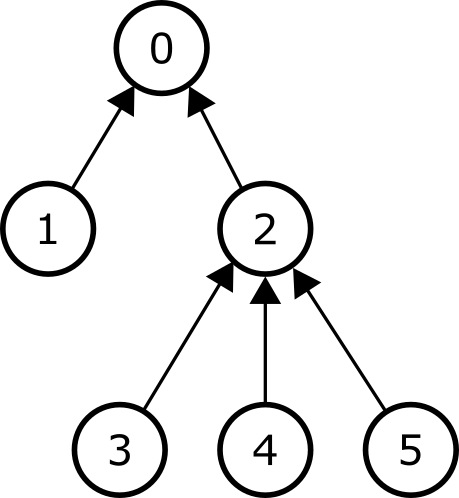
\includegraphics{subtrees.png}

Each vertex is assigned a nonnegative integer \textbf{weight}. We denote
the weight of vertex \(i\) (\(0 \leq i < N\)) by \(W[i]\).

Your task is to write a program that will answer \(Q\) queries, each
specified by a pair of positive integers \((L, R)\). The answer to the
query should be computed as follows.

Consider assigning an integer, called a \textbf{coefficient}, to each
vertex of the tree. Such an assignment is described by a sequence
\(C[0], \ldots, C[N-1]\), where \(C[i]\) (\(0 \leq i < N\)) is the
coefficient assigned to vertex \(i\). Let us call this sequence a
\textbf{coefficient sequence}. Note that the elements of the coefficient
sequence can be negative, \(0\), or positive.

For a query \((L, R)\), a coefficient sequence is called \textbf{valid}
if, for every vertex \(i\) (\(0 \leq i < N\)), the following condition
holds: the sum of the coefficients of the vertices in the subtree of
vertex \(i\) is not less than \(L\) and not greater than \(R\).

For a given coefficient sequence \(C[0], \ldots, C[N-1]\), the
\textbf{cost} of a vertex \(i\) is \(|C[i]| \cdot W[i]\), where
\(|C[i]|\) denotes the absolute value of \(C[i]\). Finally, the
\textbf{total cost} is the sum of the costs of all vertices. Your task
is to compute, for each query, the \textbf{minimum total cost} that can
be attained by some valid coefficient sequence.

It can be shown that for any query, at least one valid coefficient
sequence exists.

\hypertarget{implementation-details}{%
\subsection{Implementation Details}\label{implementation-details}}

You should implement the following two procedures:

\begin{verbatim}
void init(std::vector&lt;int&gt; P, std::vector&lt;int&gt; W)
\end{verbatim}

\begin{itemize}
\tightlist
\item
  \(P\), \(W\): arrays of integers of length \(N\) specifying the
  parents and the weights.
\item
  This procedure is called exactly once in the beginning of the
  interaction between the grader and your program in each test case.
\end{itemize}

\begin{verbatim}
long long query(int L, int R)
\end{verbatim}

\begin{itemize}
\tightlist
\item
  \(L\), \(R\): integers describing a query.
\item
  This procedure is called \(Q\) times after the invocation of
  \texttt{init} in each test case.
\item
  This procedure should return the answer to the given query.
\end{itemize}

\hypertarget{constraints}{%
\subsection{Constraints}\label{constraints}}

\begin{itemize}
\tightlist
\item
  \(1 \leq N \leq 200\,000\)
\item
  \(1 \leq Q \leq 100\,000\)
\item
  \(P[0] = -1\)
\item
  \(0 \leq P[i] < i\) for each \(i\) such that \(1 \leq i < N\)
\item
  \(0 \leq W[i] \leq 1\,000\,000\) for each \(i\) such that
  \(0 \leq i < N\)
\item
  \(1 \leq L \leq R \leq 1\,000\,000\) in each query
\end{itemize}

\hypertarget{subtasks}{%
\subsection{Subtasks}\label{subtasks}}

\begin{longtable}[]{@{}ccl@{}}
\toprule
Subtask & Score & Additional Constraints\tabularnewline
\midrule
\endhead
1 & \(10\) & \(Q \leq 10\); \(W[P[i]] \leq W[i]\) for each \(i\) such
that \(1 \leq i < N\)\tabularnewline
2 & \(13\) & \(Q \leq 10\); \(N \leq 2\,000\)\tabularnewline
3 & \(18\) & \(Q \leq 10\); \(N \leq 60\,000\)\tabularnewline
4 & \(7\) & \(W[i] = 1\) for each \(i\) such that
\(0 \leq i < N\)\tabularnewline
5 & \(11\) & \(W[i] \leq 1\) for each \(i\) such that
\(0 \leq i < N\)\tabularnewline
6 & \(22\) & \(L = 1\)\tabularnewline
7 & \(19\) & No additional constraints.\tabularnewline
\bottomrule
\end{longtable}

\hypertarget{examples}{%
\subsection{Examples}\label{examples}}

Consider the following calls:

\begin{verbatim}
init([-1, 0, 0], [1, 1, 1])
\end{verbatim}

The tree consists of \(3\) vertices, the root and its \(2\) children.
All vertices have weight \(1\).

\begin{verbatim}
query(1, 1)
\end{verbatim}

In this query \(L = R = 1\), which means the sum of coefficients in
every subtree must be equal to \(1\). Consider the coefficient sequence
\([-1, 1, 1]\). The tree and the corresponding coefficients (in shaded
rectangles) are illustrated below.

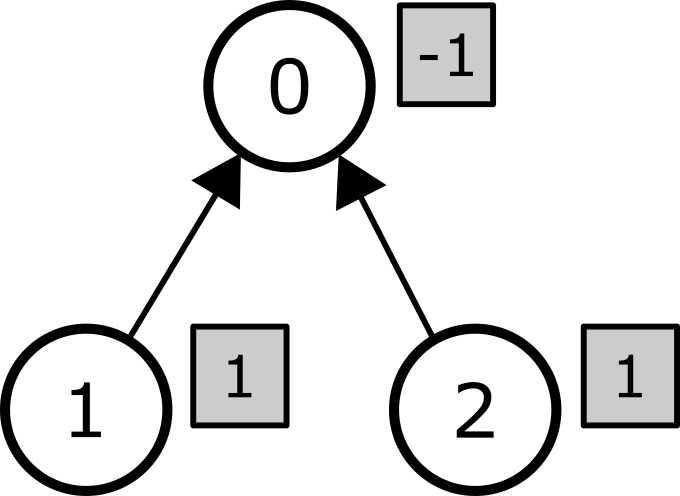
\includegraphics{ex1.png}

For every vertex \(i\) (\(0 \leq i < 3\)), the sum of the coefficients
of all vertices in the subtree of \(i\) is equal to \(1\). Hence, this
coefficient sequence is valid. The total cost is computed as follows:

\begin{longtable}[]{@{}cccc@{}}
\toprule
Vertex & Weight & Coefficient & Cost\tabularnewline
\midrule
\endhead
0 & 1 & -1 & \(\mid -1 \mid \cdot 1 = 1\)\tabularnewline
1 & 1 & 1 & \(\mid 1 \mid \cdot 1 = 1\)\tabularnewline
2 & 1 & 1 & \(\mid 1 \mid \cdot 1 = 1\)\tabularnewline
\bottomrule
\end{longtable}

Therefore the total cost is \(3\). This is the only valid coefficient
sequence, therefore this call should return \(3\).

\begin{verbatim}
query(1, 2)
\end{verbatim}

The minimum total cost for this query is \(2\), and is attained when the
coefficient sequence is \([0, 1, 1]\).

\hypertarget{sample-grader}{%
\subsection{Sample Grader}\label{sample-grader}}

Input format:

\begin{verbatim}
N
P[1]  P[2] ...  P[N-1]
W[0]  W[1] ...  W[N-2] W[N-1]
Q
L[0]  R[0]
L[1]  R[1]
...
L[Q-1]  R[Q-1]
\end{verbatim}

where \(L[j]\) and \(R[j]\) (for \(0 \leq j < Q\)) are the input
arguments in the \(j\)-th call to \texttt{query}. Note that the second
line of the input contains \textbf{only \(N-1\) integers}, as the sample
grader does not read the value of \(P[0]\).

Output format:

\begin{verbatim}
A[0]
A[1]
...
A[Q-1]
\end{verbatim}

where \(A[j]\) (for \(0 \leq j < Q\)) is the value returned by the
\(j\)-th call to \texttt{query}.
